\chapter{Misturar e dissolver}\label{ch:g2:mixing-and-dissolving}

Um cubinho de açúcar cai numa xícara de chá quente. Uma colher mexe, o
cubinho se desmancha e, depois de um instante, não sobra mais nada para
ver: o chá parece exatamente igual a antes. Mesmo assim, agora o chá
está doce. O açúcar não foi embora --- ele está escondido no chá. Este
capítulo fala de juntar coisas, e das coisas que parecem sumir quando
fazemos isso.

\begin{omfigure}
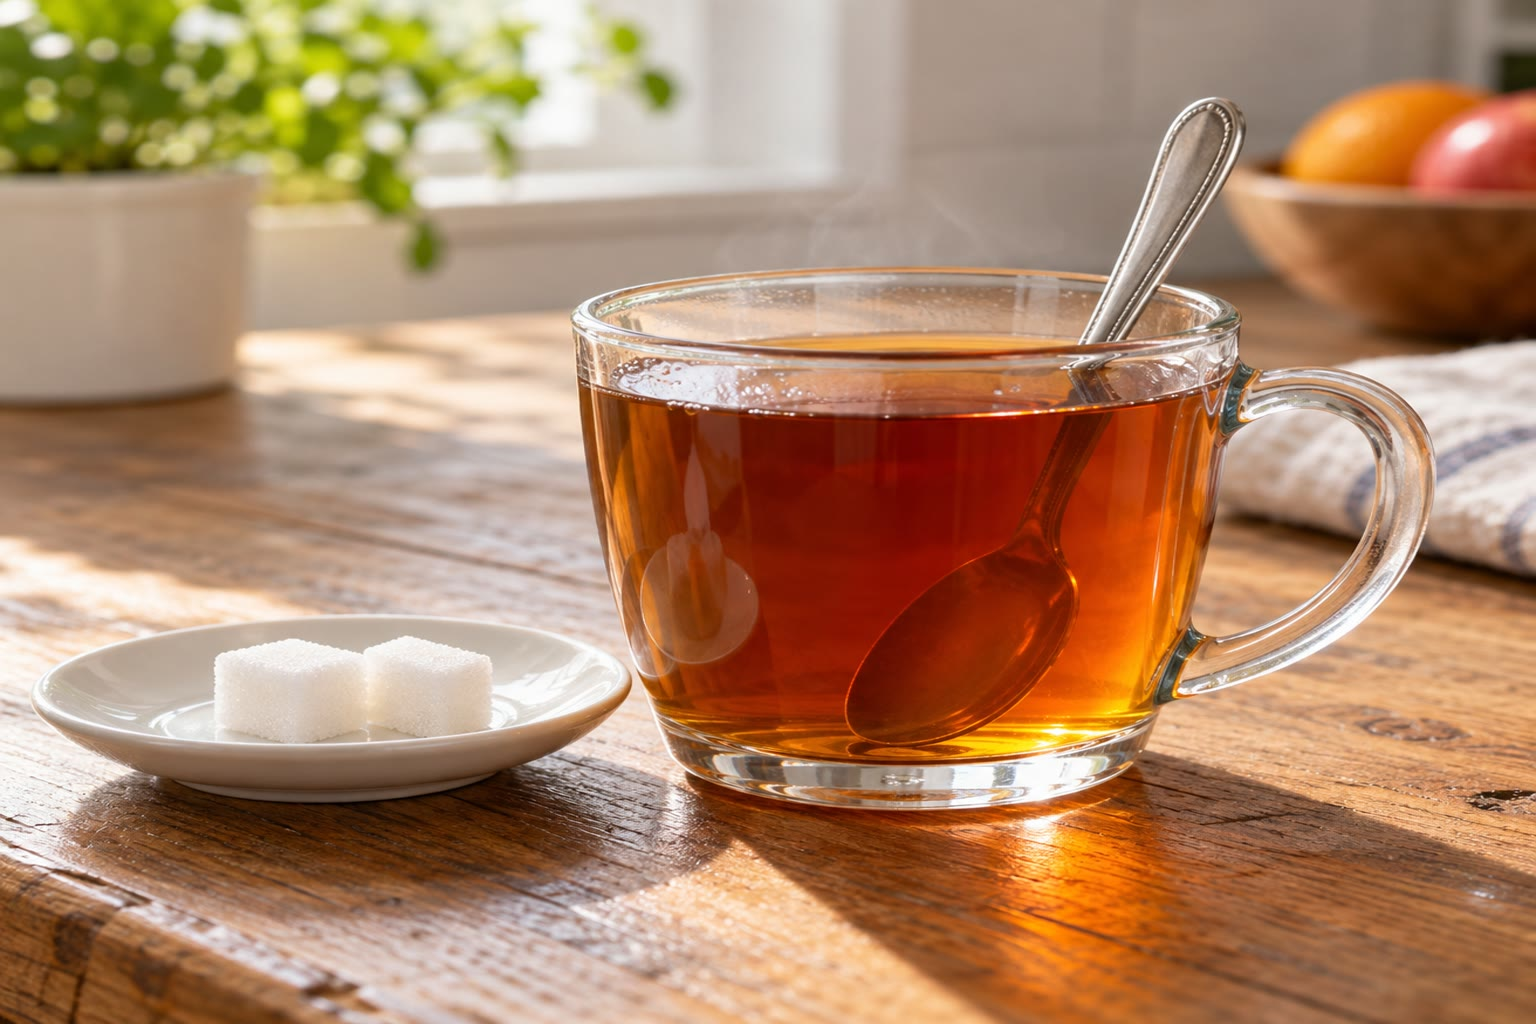
\includegraphics[width=0.55\linewidth]{images/book1/ai/g2-tea-sugar.jpg}

{\small Uma xícara de chá e dois cubinhos de açúcar. Depois de mexido, o
açúcar some da vista, mas não do gosto.}
\end{omfigure}

\section{Juntar coisas}

\begin{definition}[Misturar]\label{def:g2:mixing-and-dissolving:mix}
\emph{Misturar}\index{misturar} é juntar coisas diferentes e, muitas
vezes, mexê-las. O que obtemos é uma mistura dessas coisas.
\end{definition}

\begin{example}[Uma tigela de granola]\label{ex:g2:mixing-and-dissolving:muesli}
Aveia, uvas-passas, castanhas e sementes são despejadas numa mesma
tigela: isso é uma mistura. Olhando de perto, ainda dá para ver cada
ingrediente e tirá-lo de novo com os dedos --- uma passa continua sendo
uma passa, uma castanha continua sendo uma castanha.
\end{example}

\begin{example}[Xarope na água]\label{ex:g2:mixing-and-dissolving:syrup}
Dois líquidos também podem ser \omterm{def:g2:mixing-and-dissolving:mix}{misturados}. Um xarope vermelho despejado
num copo de água desce fazendo caracóis de cor; depois de mexer, o copo
inteiro fica cor-de-rosa por igual. A olho nu, já não dá para distinguir
o xarope da água.
\end{example}

\begin{omfigure}
\begin{minipage}[t]{0.48\linewidth}\centering
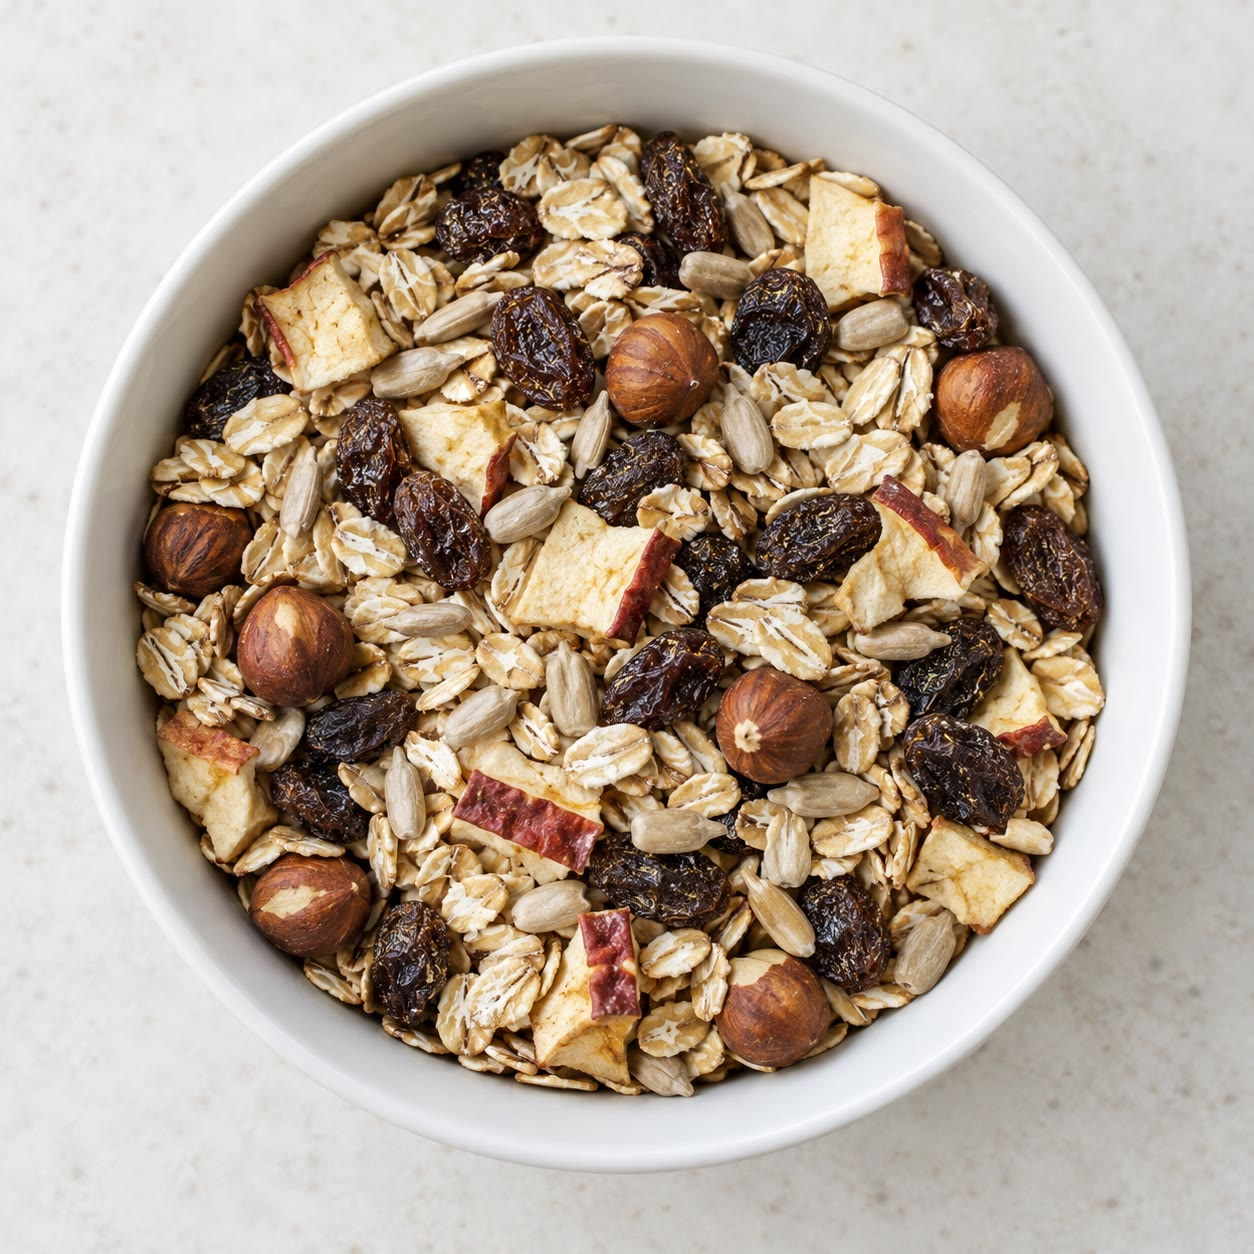
\includegraphics[width=\linewidth,height=4.6cm,keepaspectratio]{images/book1/ai/g2-muesli.jpg}

{\small Granola: uma mistura em que ainda dá para ver cada parte.}
\end{minipage}\hfill
\begin{minipage}[t]{0.48\linewidth}\centering
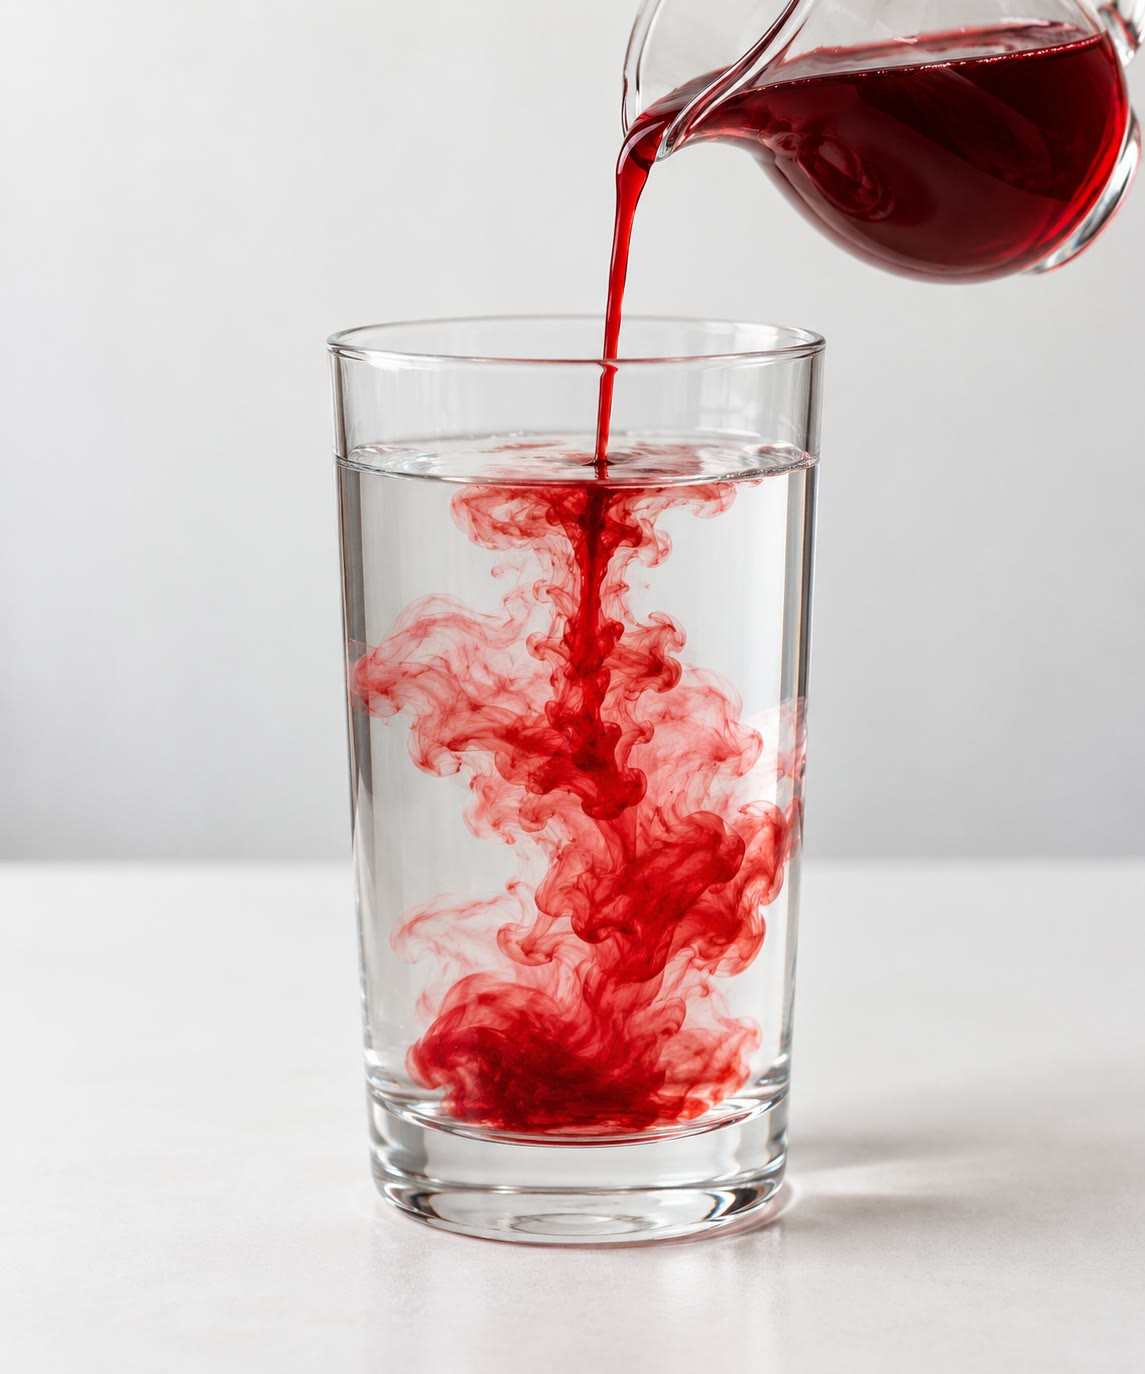
\includegraphics[width=\linewidth,height=4.6cm,keepaspectratio]{images/book1/ai/g2-syrup-in-water.jpg}

{\small Xarope despejado na água: dois líquidos se \omterm{def:g2:mixing-and-dissolving:mix}{misturando}.}
\end{minipage}
\end{omfigure}

\begin{remark}[Misturar não destrói nada]\label{rem:g2:mixing-and-dissolving:nothing-lost}
Quando \omterm{def:g2:mixing-and-dissolving:mix}{misturamos} coisas, nada se perde e nada de novo é fabricado. A
aveia, as passas e as castanhas continuam todas na tigela. Um capítulo
mais adiante mostra como separar de novo uma mistura.
\end{remark}

\section{Coisas que se dissolvem}

\begin{definition}[Dissolver e solução]\label{def:g2:mixing-and-dissolving:dissolve}
Um sólido \emph{se dissolve}\index{dissolver} na água quando, \omterm{def:g2:mixing-and-dissolving:mix}{misturado}
à água e mexido, ele some da vista e deixa o líquido \emph{límpido},
isto é, transparente. O açúcar e o sal se dissolvem na água. O líquido
límpido que obtemos se chama
\emph{solução}\index{solucao@solução}: a água com açúcar é uma solução de
açúcar, a água salgada é uma solução de sal.
\end{definition}

\begin{example}[Um cubinho de açúcar num copo de água]\label{ex:g2:mixing-and-dissolving:cube}
Um cubinho de açúcar é colocado no fundo de um copo de água parada. Os
cantos dele amolecem, ele vai ficando menor, e umas listras onduladas
sobem dele pela água. Se mexermos, ele desaparece em menos de um minuto.
Se não mexermos, ele também desaparece, só que bem mais devagar.
\end{example}

\begin{remark}[Límpido não quer dizer incolor]\label{rem:g2:mixing-and-dissolving:clear}
O chá é marrom e a água com xarope é cor-de-rosa, mas dá para ver
através dos dois: eles são límpidos. Uma \omterm{def:g2:mixing-and-dissolving:dissolve}{solução} pode ter cor. O que uma
\omterm{def:g2:mixing-and-dissolving:dissolve}{solução} nunca tem são pedacinhos boiando nem uma camada no fundo.
\end{remark}

\begin{method}[Ele se dissolve?]\label{met:g2:mixing-and-dissolving:test}
Para descobrir se um sólido \omterm{def:g2:mixing-and-dissolving:dissolve}{se dissolve} na água:
\begin{enumerate}
  \item ponha um pouquinho do sólido num copo de água;
  \item mexa e depois espere alguns minutos;
  \item olhe através do copo:
    \begin{itemize}
      \item límpido e nada no fundo: o sólido se dissolveu;
      \item turvo, ou uma camada no fundo: o sólido não se dissolveu.
    \end{itemize}
\end{enumerate}
\end{method}

\section{Coisas que não se dissolvem}

\begin{proposition}[A areia e o giz não se dissolvem]\label{prop:g2:mixing-and-dissolving:not}
Muitos sólidos não se dissolvem na água: a areia, o giz, a terra, as
pedrinhas, a farinha. Mexidos na água, eles a deixam turva; deixados em
repouso, eles descem e se depositam no fundo, e a água de cima fica mais
límpida de novo. Por mais que a gente mexa, eles nunca desaparecem.
\end{proposition}

\begin{example}[Um pote de água barrenta]\label{ex:g2:mixing-and-dissolving:mud}
Terra do jardim sacudida num pote de água deixa a água marrom e turva.
Depois de uma hora, a terra e as pedrinhas formam uma camada escura no
fundo, algumas folhas secas boiam em cima, e a água do meio fica só um
pouco turva. A terra não se dissolveu.
\end{example}

\begin{omfigure}
\begin{minipage}[t]{0.48\linewidth}\centering
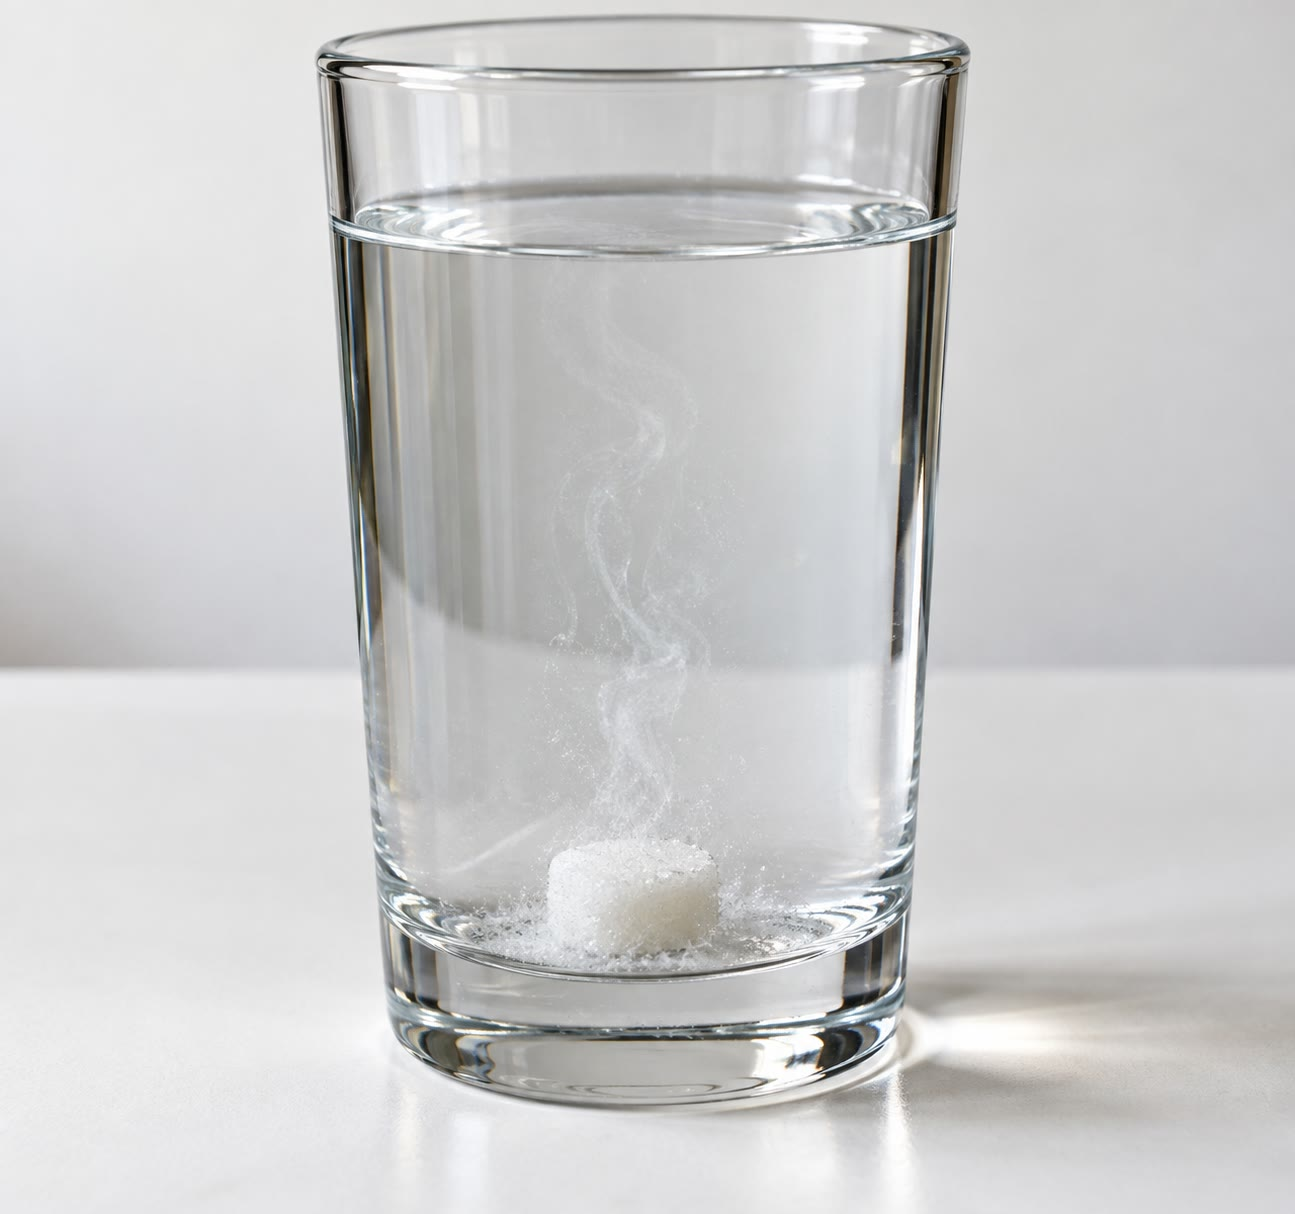
\includegraphics[width=\linewidth,height=4.6cm,keepaspectratio]{images/book1/ai/g2-sugar-cube-dissolving.jpg}

{\small O açúcar se dissolvendo: listras sobem do cubinho.}
\end{minipage}\hfill
\begin{minipage}[t]{0.48\linewidth}\centering
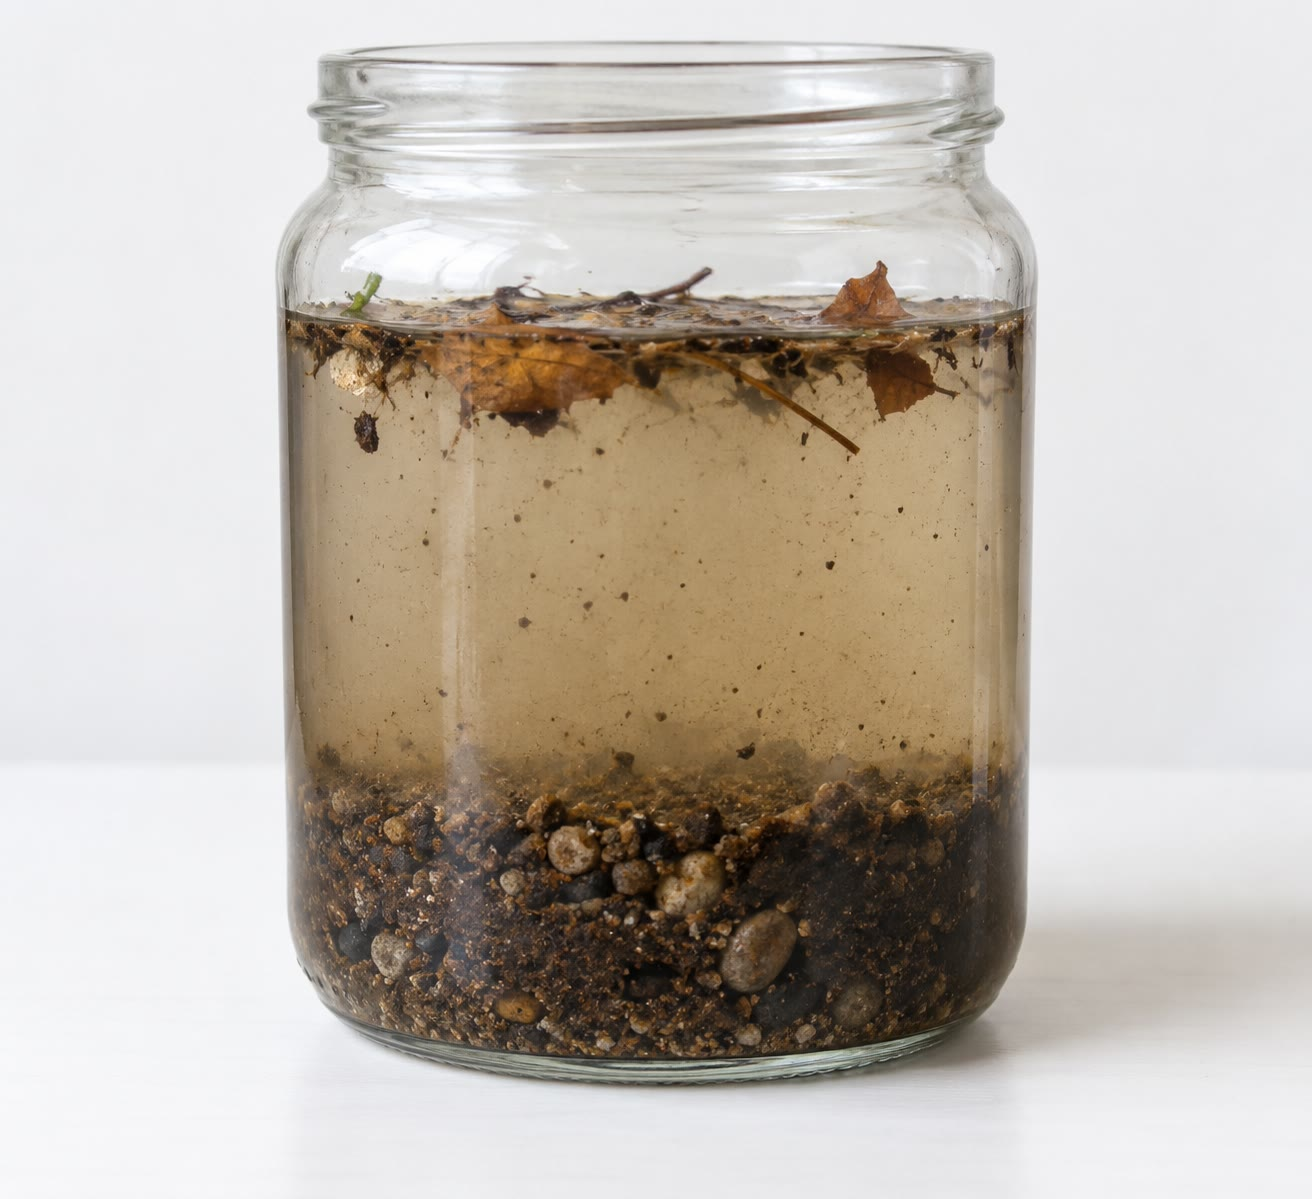
\includegraphics[width=\linewidth,height=4.6cm,keepaspectratio]{images/book1/ai/g2-muddy-jar.jpg}

{\small A terra não \omterm{def:g2:mixing-and-dissolving:dissolve}{se dissolve}: ela se deposita no fundo.}
\end{minipage}
\end{omfigure}

\begin{omfigure}
\begin{tikzpicture}[font=\small, scale=1.35]
  \pic[transform shape] at (0,0) {beaker={0.7}{omWater!70}};
  \fill[brown!55] (4.2,0) rectangle (5.8,0.22);
  \pic[transform shape] at (5,0) {beaker={0.7}{brown!12}};
  \fill[brown!55] (4.2,0) rectangle (5.8,0.22);
  \draw[omGlass, line width=0.7pt] (4.2,0.22) -- (4.2,0) -- (5.8,0) -- (5.8,0.22);
  \foreach \x/\y in {4.4/0.32,4.75/0.45,5.1/0.3,5.5/0.5,4.6/0.7,5.3/0.8,4.9/1.0}
    \fill[brown!60] (\x,\y) circle (0.025);
  \node[align=center, anchor=north] at (0,-0.15)
    {\textbf{açúcar} na água, mexido:\\ límpido, nada no fundo};
  \node[align=center, anchor=north] at (5,-0.15)
    {\textbf{areia} na água, mexida:\\ turvo, uma camada no fundo};
  \draw[<-, omProp, thick] (6.0,0.11) -- (7.0,0.11)
    node[right, text=black] {a areia};
\end{tikzpicture}

{\small O teste do \cref{met:g2:mixing-and-dissolving:test}: o açúcar
\omterm{def:g2:mixing-and-dissolving:dissolve}{se dissolve}, a areia não.}
\end{omfigure}

\section{O que se dissolve continua lá}

\begin{proposition}[Um sólido dissolvido continua na água]\label{prop:g2:mixing-and-dissolving:still-there}
Quando um sólido \omterm{def:g2:mixing-and-dissolving:dissolve}{se dissolve}, ele não some: ele fica espalhado por toda
a água, em pedacinhos pequenos demais para serem vistos. Duas pistas
mostram que ele continua lá:
\begin{itemize}
  \item o chá adoçado tem gosto doce, e a água do mar tem gosto salgado;
  \item quando a água seca, o sólido fica para trás.
\end{itemize}
\end{proposition}

\begin{remark}[No laboratório não se prova nada]\label{rem:g2:mixing-and-dissolving:no-tasting}
Sabemos que o chá é doce porque o chá é um alimento. Num laboratório,
ninguém nunca prova nada, nem mesmo um líquido que parece água: a
segunda pista, deixar a água secar, é a que os químicos usam.
\end{remark}

\begin{example}[O sal do mar]\label{ex:g2:mixing-and-dissolving:salt-pans}
Em alguns litorais ensolarados, a água do mar é levada para tanques
largos e rasos. Dia após dia, o sol seca a água. O que sobra no fundo é
um sal branco, que é juntado em montes com um rodo: o sal que estava
dissolvido no mar. O sal da mesa muitas vezes vem desses tanques, as
salinas.
\end{example}

\begin{omfigure}
\begin{tikzpicture}[font=\small, scale=1.25]
  % day 1: a saucer of salty water
  \fill[omWater!80] (0,0.18) ellipse (1.25 and 0.22);
  \draw[omGlass, line width=0.7pt] (-1.5,0.3) .. controls (-1.2,-0.15) and (1.2,-0.15) .. (1.5,0.3);
  \draw[omGlass, line width=0.5pt] (0,0.3) ellipse (1.5 and 0.28);
  \node[align=center, anchor=north] at (0,-0.35) {um pires de\\ água salgada};
  % the sun
  \fill[ocYellow] (3.4,1.45) circle (0.28);
  \foreach \a in {0,45,...,315}
    \draw[ocYellow!90!orange, thick] ($(3.4,1.45)+(\a:0.36)$) -- ($(3.4,1.45)+(\a:0.52)$);
  \draw[->, thick, omProp] (2.0,0.3) -- (4.8,0.3)
    node[midway, below, text=black, align=center] {alguns dias de\\ sol depois};
  % later: a white crust
  \begin{scope}[xshift=6.3cm]
    \draw[omGlass, line width=0.7pt] (-1.5,0.3) .. controls (-1.2,-0.15) and (1.2,-0.15) .. (1.5,0.3);
    \draw[omGlass, line width=0.5pt] (0,0.3) ellipse (1.5 and 0.28);
    \foreach \x/\y in {-0.9/0.12,-0.6/0.2,-0.3/0.08,0/0.18,0.3/0.1,0.6/0.2,0.9/0.12,
                       -0.45/0.28,0.15/0.27,0.75/0.3,-0.75/0.31}
      \fill[white, draw=black!45, line width=0.2pt] (\x,\y) rectangle ++(0.11,0.07);
    \node[align=center, anchor=north] at (0,-0.35) {sem água:\\ sal branco};
  \end{scope}
\end{tikzpicture}

{\small A água seca; o sal que estava dissolvido nela fica para
trás.}
\end{omfigure}

\begin{omfigure}
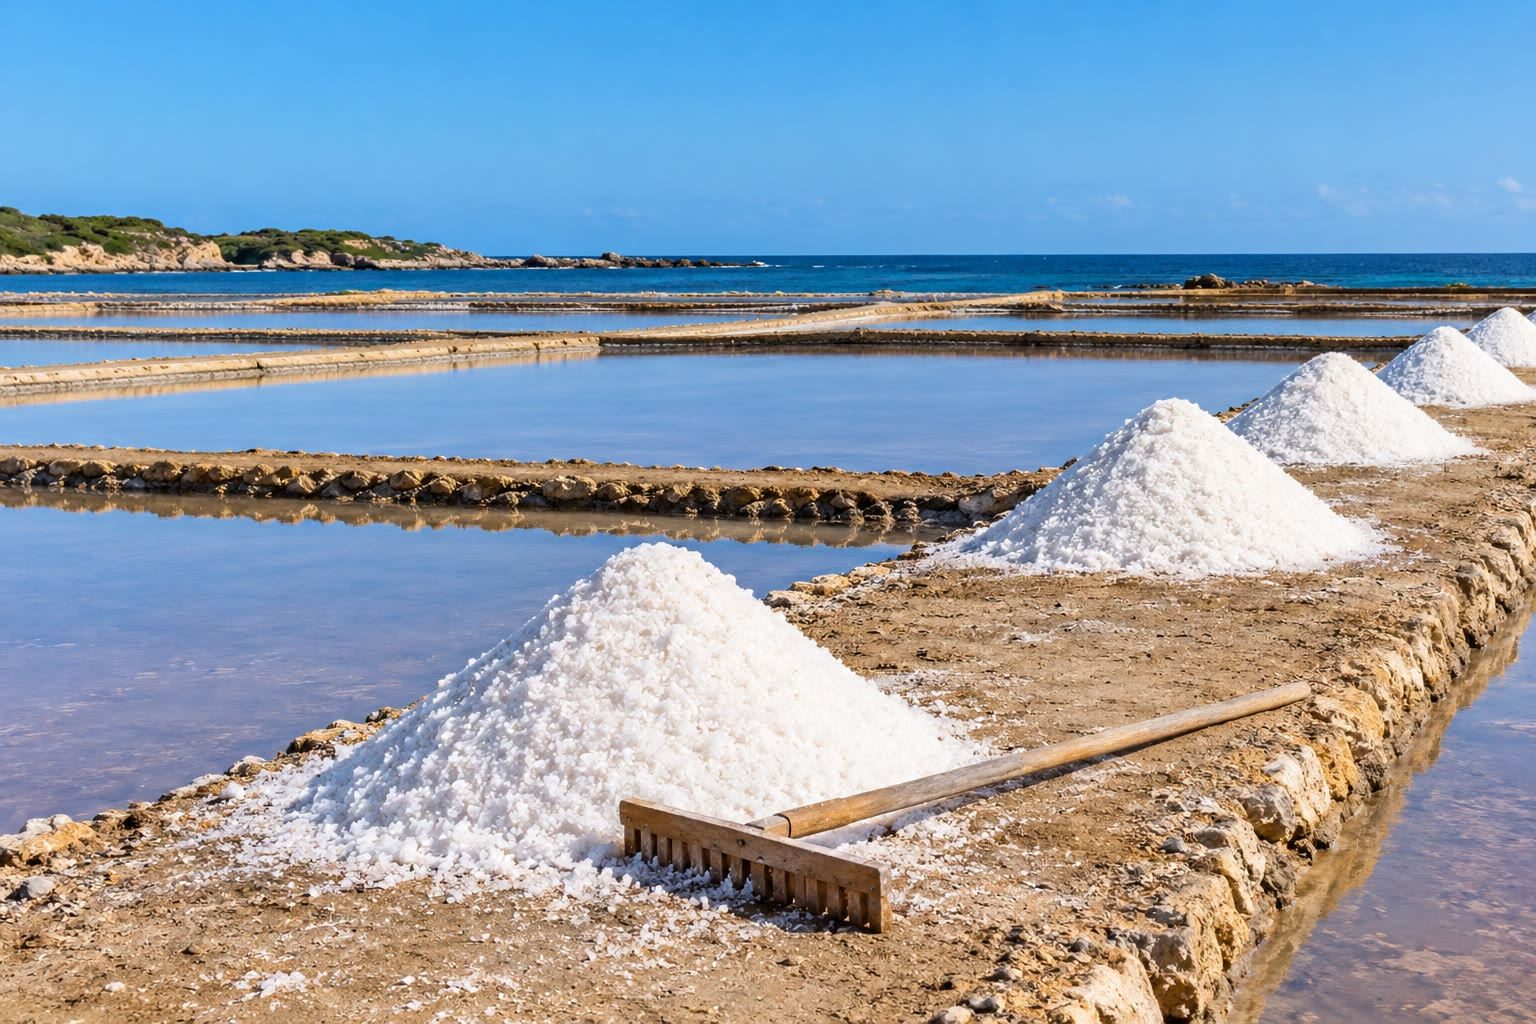
\includegraphics[width=0.62\linewidth]{images/book1/ai/g2-salt-pans.jpg}

{\small Salinas à beira-mar: o sol seca a água, e o sal fica em montes
brancos.}
\end{omfigure}

\begin{remark}[Dissolver não é derreter]\label{rem:g2:mixing-and-dissolving:not-melting}
Muita gente diz que o açúcar ``derrete'' no chá. Não é verdade: derreter
é o que um cubo de gelo faz no sol, quando vira líquido sozinho, sem
precisar de água. O açúcar no chá precisa da água, e o açúcar continua
nela, espalhado. A palavra certa é \emph{\omterm{def:g2:mixing-and-dissolving:dissolve}{dissolver}}.
\end{remark}

\section{Exercícios}

\begin{exercise}[$\star$]\label{exo:g2:mixing-and-dissolving:1}
Quais destes sólidos se dissolvem na água, e quais não? Açúcar, areia,
sal, giz, pedrinhas.
\end{exercise}

\begin{exercise}[$\star$]\label{exo:g2:mixing-and-dissolving:2}
O que é uma \omterm{def:g2:mixing-and-dissolving:dissolve}{solução}? Dê dois exemplos deste capítulo.
\end{exercise}

\begin{exercise}[$\star$]\label{exo:g2:mixing-and-dissolving:3}
Uma tigela de granola é uma mistura? Ainda dá para ver cada uma das
partes dela?
\end{exercise}

\begin{exercise}[$\star$]\label{exo:g2:mixing-and-dissolving:4}
Um pó branco é mexido num copo de água. Depois de alguns minutos, a
água está turva e uma camada branca se formou no fundo. O pó se
dissolveu? Explique usando o
\cref{met:g2:mixing-and-dissolving:test}.
\end{exercise}

\begin{exercise}[$\star$]\label{exo:g2:mixing-and-dissolving:5}
Um copo de água com xarope é cor-de-rosa. Ele é límpido? Ele é incolor?
É uma \omterm{def:g2:mixing-and-dissolving:dissolve}{solução}?
\end{exercise}

\begin{exercise}[$\star$]\label{exo:g2:mixing-and-dissolving:6}
Depois de mexer, não dá mais para ver açúcar nenhum numa xícara de chá.
Dê a pista que mostra que o açúcar continua lá.
\end{exercise}

\begin{exercise}[$\star$]\label{exo:g2:mixing-and-dissolving:7}
Nas salinas, o que o sol leva embora, e o que fica para trás?
\end{exercise}

\begin{exercise}[$\star$]\label{exo:g2:mixing-and-dissolving:8}
O Tom diz: ``O açúcar derreteu no meu chá.'' Que palavra ele deveria
usar no lugar dessa, e por quê?
\end{exercise}

\begin{exercise}[$\star\star$]\label{exo:g2:mixing-and-dissolving:9}
Olhe a figura dos dois béqueres. Sem ler as palavras embaixo deles,
como você sabe qual béquer tem a areia?
\end{exercise}

\begin{exercise}[$\star\star$]\label{exo:g2:mixing-and-dissolving:10}
Uma gota de água da torneira seca num prato preto e deixa uma pequena
marca branca em forma de anel. O que isso nos diz sobre a água da
torneira?
\end{exercise}

\begin{exercise}[$\star\star$]\label{exo:g2:mixing-and-dissolving:11}
No laboratório, uma professora tem dois copos de líquido límpido e
incolor: um tem água pura, o outro tem água salgada. Ninguém pode
prová-los. Como ela pode descobrir qual é qual?
\end{exercise}
